\documentclass{article}
\usepackage[ampersand]{easylist}
\usepackage{amsmath}
\usepackage{graphicx}
\graphicspath{ {C:/Users/ustjo/Desktop/Investing/Stocks/canslim/weeklyStockScanner/Figures/} }
\usepackage[inline]{enumitem}
\usepackage{lscape}
\begin{document}
\title{About the Stock Scanner}
\author{KAI YIN, CHAN}
\maketitle
\section{Introduction}
The first question to answer when investing on stocks is which stock to buy? Section 1 answers this question. The second question to answer is when to buy the stock? Section 2 answers this question.

\section{Which stock to buy?}
There are ten criteria included in the stock scanner.

First of all, earnings per share (EPS) in the latest quarter should be up at least 25 \% versus the same quarter a year ago. It may imply the profitability of the company of concern improved significantly. Diluted EPS excluding extraordinary items is used.

Secondly, earning per share in current quarter should be greater than zero. This ensures the company of concern is not losing money and increases the probability that the earning growth (criteria 1) may continue.

Thirdly. sales in the latest quarter should be up at least 25 \% versus the same quarter a year ago. While EPS may be affected by number of shares outstanding and therefore may not reflect the whole picture of profitability, sales figure can strengthen the confidence that the company is indeed profitable.

After looking at quarterly data, a year-by-year earnings increase for each of the last 3 years is required. Meaning, EPS TTM (Trailing 12 months, i.e. the past 12 months) should be greater than EPS Y1. EPS Y1 should be greater than EPS Y2. And EPS Y2 should be greater than EPS Y3. This may imply the profitability of the company does not show a downtrend.

Apart from annual earnings increase, the average annual EPS growth rate should be at least 25 \% over the last 5 years. It may imply the profitability of the company improved significantly over the years. Again diluted EPS excluding extraordinary items is used.

The next criteria is that the consensus earnings estimate for the next year should be higher than the current year. A consensus estimate is a figure based on the combined estimates of the analysts. This leverage on different analysis models to further improve our confidence that the profitability of the company is growing.

Furthermore, return on equity (ROE) should be greater than 17 \%. Compared to EPS, return on equity is a direct measure of company's profitability. It measures the return generated per unit of shareholders' equity.

Cash flow is also a concern. It is required that Cash flow per share (TTM) is greater than earnings per share (TTM) by at least 20 \%

The above 8 criteria focuses on the profitability of the company of concern. It is believed that company's profitability is correlated to stock price. Therefore, the scanner uses both annual and quarterly EPS, sales data, and ROE as well as cash flow per share to increase the prediction confidence of short term profitability growth and thus improve the likelihood that the stock price will rise.

At last, it is suggested to stand behind giant. Therefore, it is required that the company of concern should have more than 10 institutional owners, but the institutional ownership percentage should be lower than 35 \% to avoid potential price manipulation.

\section{When to buy the stock?}
\subsection{Cup with a handle}
If a particular stock that passes the scanning in Section 2 and contains the bellow features, buy the stock at the top of the handle plus \$0.1.
\NewList
\begin{easylist}
& The pattern should start with a prior uptrend.
& The base length should be at least 7 weeks.
& The  handle length should be at least 1 week.
& The correction to form the base should be at most 30\%.
& the correction to form the handle should be at most 12\%.
& the handle size should not be greater than half of tha of the cup.
& the shape of the cup should be U-Shape.
& the volume within the cup should be U-Shape.
& the volume in the bottom of the handle should be the lowest.
\end{easylist}

Please check Figure \ref{fig:Cup with a handle}

\begin{figure}[h]
\centering
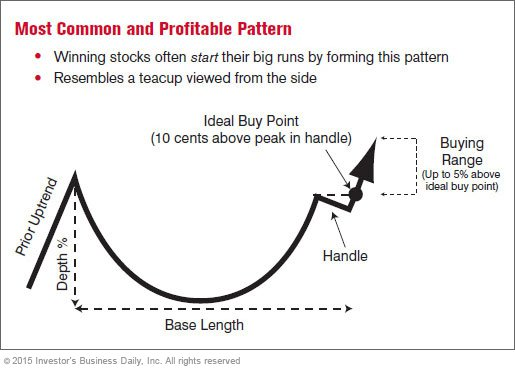
\includegraphics[width=\textwidth]{cupWithAHandle.png}
\caption{Cup with a handle}
\label{fig:Cup with a handle}
\end{figure}

\subsection{Double bottom}
If a particular stock that passes the scanning in Section 2 and contains the bellow features, buy the stock at the top of the second cup plus \$0.1.
\NewList
\begin{easylist}
& the second bottom should be lower than the first bottom.
& the base length (from the start of first cup to the end of second cup) should be at least 7 weeks.
& the correction to form the base should be at most 30\%.
& the shape should be W-Shape.
\end{easylist}

\subsection{Flat base}
It usually occurs after a stock has advanced off of a 'cup with handle' or 'double bottom' pattern. The 'flat base' moves straight sideways in a fairly tight price range for at least five weeks and does not correct more than 10\% to 15\%. Buy the stock at the top of the flat base plus \%0.1.
\end{document}
